\documentclass[11pt,a4paper]{article}
\usepackage[utf8]{inputenc}
\usepackage{amsmath,amssymb,amsfonts}
\usepackage{graphicx}
\usepackage{geometry}
\usepackage{booktabs}
\usepackage{hyperref}
\usepackage{color}
\usepackage{listings}
\usepackage{tikz}
\usetikzlibrary{shapes.geometric, arrows.meta, positioning}

\geometry{margin=1in}

\title{\textbf{Introduction to Quadruped Locomotion Control:\\Mathematical Foundations of the M2 Metal Quadruped}}
\date{\today}

\begin{document}

\maketitle

\begin{abstract}
This guide provides a comprehensive, beginner-friendly introduction to the mathematical and algorithmic components that power the M2 Metal quadruped trot-gait simulation. We cover coordinate frames, the Finite State Machine (FSM), foot trajectory generation via quintic polynomials, analytic inverse kinematics, leg Jacobians, contact forces, and the unique transmission-space PD actuator control geometry of the M2 Metal hardware.
\end{abstract}

\tableofcontents
\newpage

\section{Introduction and Leg Conventions}
Locomotion in a quadruped robot requires coordinating 12 actuated joints (3 per leg) to move the robot's base body (the trunk) stably through 3D space. 

\subsection{Leg Labeling and Order}
By standard convention, the legs are ordered and indexed as follows:
\begin{table}[h!]
\centering
\begin{tabular}{ccl}
\toprule
\textbf{Leg Index} & \textbf{Abbreviation} & \textbf{Name} \\
\midrule
0 & FR & Front Right \\
1 & FL & Front Left \\
2 & RR & Rear Right \\
3 & RL & Rear Left \\
\bottomrule
\end{tabular}
\caption{Leg indices used in the trot-gait controller.}
\end{table}

\subsection{Joint Configuration per Leg}
Each leg is modeled as a 3-DOF serial kinematic chain:
\begin{enumerate}
    \item \textbf{Abduction/Adduction (Hip Roll, $q_1$):} Controls lateral (side-to-side) leg movement.
    \item \textbf{Hip Pitch (Thigh, $q_2$):} Controls fore-aft (forward-back) leg movement.
    \item \textbf{Knee Pitch (Calf, $q_3$):} Controls extension/flexion of the lower leg.
\end{enumerate}

The local coordinate frame of the leg is centered at the abduction joint. The foot position relative to the hip/abduction base frame is defined as $\mathbf{X} = [x, y, z]^T$.

\section{Control Loop Architecture}

\subsection{Control Goal and Challenge}
Given a desired body velocity $(v_{x,ref}, v_{y,ref}, \dot{\psi}_{ref})$, the controller must compute 12 joint torques every timestep so the robot walks at those speeds while staying upright. The challenge is bridging the gap between high-level velocity commands and low-level joint torques. The solution decomposes into three nested layers:

\begin{table}[h!]
\centering
\begin{tabular}{lll}
\toprule
\textbf{Layer} & \textbf{Question Answered} & \textbf{Key Tools} \\
\midrule
1 $\cdot$ Gait Planning & Where does each foot land next? & Finite-state machine, Raibert heuristic \\
2 $\cdot$ Kinematics & How must joints move to put feet there? & Quintic polynomial, IK, Jacobian \\
3 $\cdot$ Dynamics & What torques produce the required forces? & Newton-Euler wrench balance, PD, $-\mathbf{J}^T\mathbf{F}$ \\
\bottomrule
\end{tabular}
\caption{Nested layers of the quadruped locomotion pipeline.}
\end{table}

\subsection{Why Each Tool Is Necessary}
\begin{table}[h!]
\centering
\begin{tabular}{lp{10cm}}
\toprule
\textbf{Tool} & \textbf{Role in the Pipeline} \\
\midrule
Raibert heuristic & The only place $v_{ref}$ enters the leg geometry — maps speed to step length. \\
Quintic polynomial & Guarantees zero velocity/acceleration at lift-off and touch-down, eliminating impact spikes. \\
Inverse kinematics & Solves the nonlinear geometry: Cartesian foot target $\to$ 3 joint angles. \\
Forward kinematics & Finds foot positions and COM in world frame — needed to build the lever-arm matrix $\mathbf{A}$. \\
Jacobian & Bridges two domains: Cartesian velocity $\to$ joint velocity, and foot force $\to$ joint torque. \\
Newton-Euler + $\mathbf{A}^+$ & Distributes a 6-DOF net wrench across two stance legs — pure statics, no dynamics inversion. \\
PD in joint space & Handles model error and swing-leg tracking. \\
$-\mathbf{J}^T \mathbf{F}$ feedforward & Principle of virtual work: exact joint torques to produce the desired foot force. \\
\bottomrule
\end{tabular}
\caption{Role of each mathematical tool in the pipeline.}
\end{table}

\subsection{Complete Data Flow}
The complete execution pipeline from high-level commands to low-level motor torques is shown below:

\begin{figure}[h!]
\centering
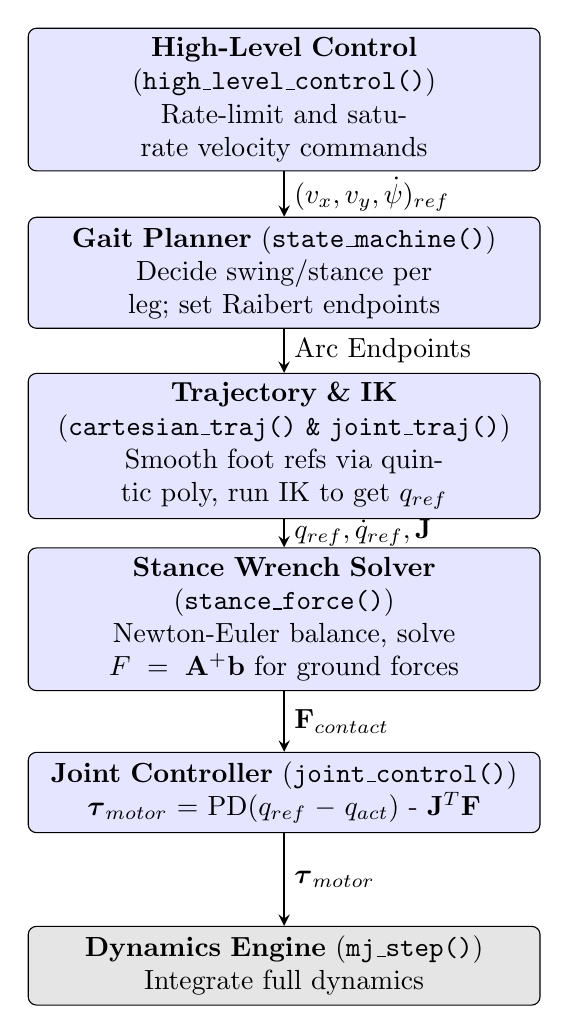
\begin{tikzpicture}[
    node distance=2.2cm,
    process/.style={rectangle, minimum width=6.5cm, minimum height=1cm, text centered, draw=black, fill=blue!10, rounded corners=3pt, text width=6cm},
    arrow/.style={thick,->,>=stealth}
]

\node (highlevel) [process] {\textbf{High-Level Control} (\texttt{high\_level\_control()})\\ Rate-limit and saturate velocity commands};
\node (fsm) [process, below of=highlevel] {\textbf{Gait Planner} (\texttt{state\_machine()})\\ Decide swing/stance per leg; set Raibert endpoints};
\node (traj) [process, below of=fsm] {\textbf{Trajectory \& IK} (\texttt{cartesian\_traj() \& joint\_traj()})\\ Smooth foot refs via quintic poly, run IK to get $q_{ref}$};
\node (stance) [process, below of=traj] {\textbf{Stance Wrench Solver} (\texttt{stance\_force()})\\ Newton-Euler balance, solve $F = \mathbf{A}^+ \mathbf{b}$ for ground forces};
\node (joint) [process, below of=stance] {\textbf{Joint Controller} (\texttt{joint\_control()})\\ $\boldsymbol{\tau}_{motor}$ = PD($q_{ref} - q_{act}$) - $\mathbf{J}^T \mathbf{F}$};
\node (mj) [process, below of=joint, fill=gray!20] {\textbf{Dynamics Engine} (\texttt{mj\_step()})\\ Integrate full dynamics};

\draw [arrow] (highlevel) -- node[anchor=west] {$(v_x, v_y, \dot{\psi})_{ref}$} (fsm);
\draw [arrow] (fsm) -- node[anchor=west] {Arc Endpoints} (traj);
\draw [arrow] (traj) -- node[anchor=west] {$q_{ref}, \dot{q}_{ref}, \mathbf{J}$} (stance);
\draw [arrow] (stance) -- node[anchor=west] {$\mathbf{F}_{contact}$} (joint);
\draw [arrow] (joint) -- node[anchor=west] {$\boldsymbol{\tau}_{motor}$} (mj);

\end{tikzpicture}
\caption{Data flow of the quadruped control pipeline executed every timestep.}
\end{figure}

\section{The Locomotion Finite State Machine (FSM)}
Locomotion is controlled by a Finite State Machine running independently for each leg. The FSM determines whether a leg should be supporting the robot's weight (stance) or moving to a new step target (swing).

\subsection{Trot Gait Timing and Coordination}
Trotting is a symmetric, diagonal gait. The legs are grouped into two diagonal pairs that move in phase:
\begin{itemize}
    \item \textbf{Diagonal Pair A:} FL (Front Left) and RR (Rear Right)
    \item \textbf{Diagonal Pair B:} FR (Front Right) and RL (Rear Left)
\end{itemize}
While Pair A is in stance (pushing the body), Pair B is in swing (stepping forward). The duration of the stance and swing phases are equal ($T_{stance} = T_{swing} = 0.15$~s), meaning the duty factor is exactly 50\%.

\subsection{FSM States and Transitions}
The trot gait uses three distinct states for each leg $i \in \{0, 1, 2, 3\}$:
\begin{itemize}
    \item \textbf{\texttt{fsm\_stand} (State 1):} A starting calibration state where all 4 feet remain planted on the ground while the trunk height slowly settles from its initial drop to the nominal walking height $z_0 = -0.32$~m.
    \item \textbf{\texttt{fsm\_stance} (State 2):} The foot is planted on the ground, acting as a support. During stance, the leg exerts vertical forces to support the trunk and linear/angular forces to drive the body.
    \item \textbf{\texttt{fsm\_swing} (State 3):} The foot is lifted from the ground and moves along a clearance arc to its next target step location.
\end{itemize}

Transitions between these states are governed by time thresholds:
\begin{enumerate}
    \item \textbf{Stand $\to$ Swing/Stance}: Triggered when $t \ge t_{stand}$ (nominal settling time).
    \begin{itemize}
        \item Diagonal Pair B (FR, RL) transitions to \textbf{\texttt{fsm\_swing}}, lifting to clearance height: $z_f = z_0 + h_{cl}$.
        \item Diagonal Pair A (FL, RR) transitions to \textbf{\texttt{fsm\_stance}}, remaining at ground level: $z_f = z_0$.
    \end{itemize}
    \item \textbf{Stance $\to$ Swing}: Triggered when $t \ge t_{fsm} + T_{step}$ while in stance. The foot lifts off and travels from behind the hip to ahead of the hip. The landing targets are computed using the \textbf{Raibert Heuristic}:
    \begin{equation}
    x_{target} = \frac{T_{step}}{2} v_{x,ref}, \quad y_{target} = \frac{T_{step}}{2} v_{y,ref}
    \end{equation}
    The term $\frac{T_{step}}{2} v_{ref}$ represents the \textit{symmetry term} — if the foot lands here, the body moves symmetrically over the foot during stance, yielding zero net acceleration. Thus, the FSM sets the endpoints:
    \begin{align}
    x_i &= -0.5 v_{x,ref} T_{step}, \quad x_f = 0.5 v_{x,ref} T_{step} \\
    y_i &= -0.5 v_{y,ref} T_{step}, \quad y_f = 0.5 v_{y,ref} T_{step} \\
    z_i &= z_0, \quad z_f = z_0 + h_{cl}
    \end{align}
    To coordinate turning, a yaw rate coupling term with lever arm $c = 0.183$~m is added to the lateral coordinates:
    \begin{align}
    y_i &\leftarrow y_i \mp 0.5 c \dot{\psi}_{ref} T_{step} \\
    y_f &\leftarrow y_f \pm 0.5 c \dot{\psi}_{ref} T_{step}
    \end{align}
    where the upper sign is for the front legs (FL, FR) and the lower sign is for the rear legs (RL, RR).
    
    \item \textbf{Swing $\to$ Stance}: Triggered when $t \ge t_{fsm} + T_{step}$ while in swing. The foot plants and moves backward relative to the hip:
    \begin{align}
    x_i &= 0.5 v_{x,ref} T_{step}, \quad x_f = -0.5 v_{x,ref} T_{step} \\
    y_i &= 0.5 v_{y,ref} T_{step}, \quad y_f = -0.5 v_{y,ref} T_{step} \\
    z_i &= z_0, \quad z_f = z_0
    \end{align}
    The yaw coupling is applied symmetrically to match the stance motion:
    \begin{align}
    y_i &\leftarrow y_i \pm 0.5 c \dot{\psi}_{ref} T_{step} \\
    y_f &\leftarrow y_f \mp 0.5 c \dot{\psi}_{ref} T_{step}
    \end{align}
\end{enumerate}

\section{Cartesian Foot Trajectory Generation}
When a leg is in the swing phase, the foot must move smoothly from its liftoff position $\mathbf{p}_i = [x_i, y_i, z_i]^T$ to its Raibert touchdown position $\mathbf{p}_f = [x_f, y_f, z_f]^T$. To avoid high impact forces, the foot must lift off and touch down with \textbf{zero velocity} and \textbf{zero acceleration}.

\subsection{Quintic (5th-Order) Polynomials}
To satisfy these boundary conditions, we use a 5th-order polynomial to interpolate the footprint position. Let $s(\tau)$ be a normalized scaling parameter where $\tau = \frac{t}{T} \in [0, 1]$:
\begin{equation}
s(\tau) = 10\tau^3 - 15\tau^4 + 6\tau^5
\end{equation}
Differentiating with respect to time gives the normalized velocity $\dot{s}(\tau)$ and acceleration $\ddot{s}(\tau)$:
\begin{align}
\dot{s}(\tau) &= \frac{1}{T} (30\tau^2 - 60\tau^3 + 30\tau^4) \\
\ddot{s}(\tau) &= \frac{1}{T^2} (60\tau - 180\tau^2 + 120\tau^3)
\end{align}

At the boundaries:
\begin{itemize}
    \item $\tau = 0 \implies s = 0, \dot{s} = 0, \ddot{s} = 0$ (Smooth lift-off)
    \item $\tau = 1 \implies s = 1, \dot{s} = 0, \ddot{s} = 0$ (Smooth touchdown)
\end{itemize}

For $x$ and $y$, the reference position and velocity at time $t$ are:
\begin{align}
x_{ref}(t) &= x_i + (x_f - x_i) s(\tau) \\
\dot{x}_{ref}(t) &= (x_f - x_i) \dot{s}(\tau)
\end{align}

\subsection{Two-Segment Vertical Clearance Arc}
To clear obstacles, the foot height $z$ must lift up to a clearance height $h_{cl} = 0.06$~m at mid-swing and return to the ground. Doing this in a single polynomial would create a velocity discontinuity. Thus, the swing is split into two halves:
\begin{enumerate}
    \item \textbf{First Half ($0 \le t \le 0.5 T$):} The foot rises from $z_i$ to $z_{max} = z_i + h_{cl}$.
    \item \textbf{Second Half ($0.5 T < t \le T$):} The foot descends from $z_{max}$ to $z_f$.
\end{enumerate}
Each segment is solved using a separate quintic polynomial to guarantee smooth velocity matchings at the apex.

\section{Leg Kinematics and Jacobian Mapping}

\subsection{Analytic Inverse Kinematics (IK)}
The joint angles $\mathbf{q} = [q_1, q_2, q_3]^T$ needed to place the foot at a relative Cartesian position $\mathbf{X}_{ref} = [l_x, l_y, l_z]^T$ are solved using the approximate leg geometry (Method 0), where link lengths are symmetric ($L_1 = L_2 = 0.1915$~m) and structural offsets $w$ and $dx$ are ignored to enable a fast closed-form solution.

Let the total leg length distance from the hip to the foot be:
\begin{equation}
l = \sqrt{l_x^2 + l_y^2 + l_z^2}
\end{equation}

First, the abduction joint angle $q_1$ is determined by lateral displacement $l_y$ relative to total length $l$:
\begin{equation}
q_1 = \arcsin\left(\operatorname{clip}\left(\frac{l_y}{l}, -1, 1\right)\right)
\end{equation}

Next, the knee pitch joint angle $q_3$ is solved using the law of cosines under the symmetric link assumption ($L_1 = L_2$):
\begin{equation}
q_3 = -\pi + \arccos\left(\operatorname{clip}\left(\frac{2 L_1^2 - l^2}{2 L_1^2}, -1, 1\right)\right)
\end{equation}

Finally, the hip pitch joint angle $q_2$ is calculated by subtracting the knee contribution from the pitch angle:
\begin{equation}
q_2 = -0.5 q_3 + \arcsin\left(\operatorname{clip}\left(\frac{-l_x}{l}, -1, 1\right)\right)
\end{equation}

\subsection{The Foot Jacobian}
The Jacobian matrix $\mathbf{J}(\mathbf{q})$ maps joint velocities to foot Cartesian velocities:
\begin{equation}
\dot{\mathbf{X}} = \mathbf{J}(\mathbf{q})\dot{\mathbf{q}}
\end{equation}
The joint velocity reference $\dot{\mathbf{q}}_{ref}$ is found by inverting the Jacobian:
\begin{equation}
\dot{\mathbf{q}}_{ref} = \mathbf{J}(\mathbf{q})^{-1} \dot{\mathbf{X}}_{ref}
\end{equation}
(Note: In practical implementations near singular configurations, e.g., full leg extension where $q_3 \to 0$, a damped pseudo-inverse is typically used instead of a direct inversion to prevent velocity spikes).

By the principle of virtual work, the Jacobian also maps a desired Cartesian foot force $\mathbf{F}$ to joint torques $\mathbf{\tau}$:
\begin{equation}
\mathbf{\tau} = -\mathbf{J}(\mathbf{q})^T \mathbf{F}
\end{equation}
The negative sign appears because $\mathbf{F}$ is defined as the desired \textit{ground reaction force} (the force the ground exerts on the foot). This allows us to apply direct force feedforward to push the ground during stance.

\subsection{Stance Wrench and Ground Force Allocation (Virtual Model Control)}
During the stance phase, we compute the desired virtual forces/torques (a 6-DOF wrench $\mathbf{b} \in \mathbb{R}^6$) that must be exerted on the robot's trunk to track target linear/angular velocities and keep the base level. This is known as \textbf{Virtual Model Control (VMC)}, where imaginary springs and dampers connect the trunk to the desired target state.

To ensure that velocity commands are independent of the robot's heading (e.g. forward velocity $v_x$ always means moving straight out from the "face" of the robot), the trunk velocities are decoupled from yaw:
\begin{equation}
\mathbf{v}_{body} = \mathbf{R}_z(\psi)^T \mathbf{v}_{world}, \quad \mathbf{R}_{body} = \mathbf{R}_z(\psi)^T \mathbf{R}_{world}
\end{equation}
The desired wrench $\mathbf{b}$ is then computed in this yaw-decoupled frame using proportional-derivative (PD) feedback loops on the trunk state:
\begin{equation}
\mathbf{b} = \begin{bmatrix}
K_{p,vx} (v_{x,ref} - v_x) \\
K_{p,vy} (v_{y,ref} - v_y) \\
K_{p,z} (z_{ref} - z) - K_{d,z} \dot{z} + m g \\
K_{p,\phi} (0 - \phi) - K_{d,\phi} \omega_x \\
K_{p,\theta} (0 - \theta) - K_{d,\theta} \omega_y \\
K_{p,\psi} (\dot{\psi}_{ref} - \dot{\psi})
\end{bmatrix}
\end{equation}
where:
\begin{itemize}
    \item $v_x, v_y, z$ are the trunk's linear velocities and height.
    \item $\phi, \theta, \dot{\psi}$ are the trunk's roll, pitch, and yaw rate.
    \item $m = 11.5$~kg is the robot's mass, and $g = 9.81$~m/s$^2$ is gravity.
    \item $K_p$ and $K_d$ are the tracking gains.
\end{itemize}

Since trotting relies on diagonal stance pairs, the wrench $\mathbf{b}$ must be distributed between the two active stance feet. For a given active diagonal pair (e.g., foot $A$ and foot $B$), the ground reaction force vectors $\mathbf{F}_A, \mathbf{F}_B \in \mathbb{R}^3$ are related to the trunk wrench by:
\begin{equation}
\mathbf{A} \begin{bmatrix} \mathbf{F}_A \\ \mathbf{F}_B \end{bmatrix} = \mathbf{b}
\end{equation}
where the force-to-wrench mapping matrix $\mathbf{A} \in \mathbb{R}^{6 \times 6}$ is:
\begin{equation}
\mathbf{A} = \begin{bmatrix}
\mathbf{I}_3 & \mathbf{I}_3 \\
[\mathbf{r}_A \times] & [\mathbf{r}_B \times]
\end{bmatrix}
\end{equation}
and:
\begin{itemize}
    \item $\mathbf{I}_3$ is the $3 \times 3$ identity matrix.
    \item $\mathbf{r}_A, \mathbf{r}_B \in \mathbb{R}^3$ are the position vectors from the trunk center of mass (COM) to foot $A$ and foot $B$, respectively.
    \item $[\mathbf{r} \times] \in \mathbb{R}^{3 \times 3}$ is the skew-symmetric cross-product matrix:
    \begin{equation}
    [\mathbf{r} \times] = \begin{bmatrix}
    0 & -r_z & r_y \\
    r_z & 0 & -r_x \\
    -r_y & r_x & 0
    \end{bmatrix}
    \end{equation}
\end{itemize}

Since $\mathbf{A}$ is a square matrix (for a two-leg support phase), the required contact forces are solved directly using the pseudo-inverse:
\begin{equation}
\begin{bmatrix} \mathbf{F}_A \\ \mathbf{F}_B \end{bmatrix} = \mathbf{A}^{-1} \mathbf{b}
\end{equation}
These forces are then mapped to joint torques via the Jacobians of the respective stance legs. The final torque command sent to the motors is a decomposition of two distinct components:
\begin{equation}
\boldsymbol{\tau} = \underbrace{\mathbf{J}_\theta^T \boldsymbol{\tau}_{motor}}_{\text{PD tracking (all legs)}} + \underbrace{(-\mathbf{J}^T \mathbf{F})}_{\text{Stance feedforward only}}
\end{equation}
The first term provides tracking of the swing trajectories and ground compliance via joint PD control. The second term is applied \textit{only} to legs currently in the Stance phase, exerting the required ground reaction forces to support and propel the trunk.

\section{PD Control and Transmission Geometry}
The M2 Metal does not place motors directly at the joints. Instead, motors are mounted on the trunk and drive the hip, thigh, and calf joints via low-inertia belts. This creates a mechanical coupling between the thigh and calf.

\subsection{Belt Transmission Coupling}
Because the belt driving the calf runs past the thigh joint, moving the thigh joint ($q_2$) changes the belt routing and rotates the calf. To maintain the calf angle, the calf motor must rotate. The relationship between motor angles $\mathbf{\theta} = [\theta_1, \theta_2, \theta_3]^T$ and joint angles $\mathbf{q} = [q_1, q_2, q_3]^T$ is:
\begin{align}
\theta_1 &= N_{ab} q_1 \\
\theta_2 &= N_{hip} q_2 \\
\theta_3 &= N_{knee} q_3 + N_{knee} \gamma q_2
\end{align}
where:
\begin{itemize}
    \item $N_{ab} = 8$, $N_{hip} = 8$, and $N_{knee} = 16$ are the gear reduction ratios.
    \item $\gamma = 0.5$ is the belt transmission coupling coefficient.
\end{itemize}

We can write this in matrix form using the transmission Jacobian $\mathbf{J}_{\theta}$:
\begin{equation}
\mathbf{\theta} = \mathbf{J}_{\theta} \mathbf{q} \implies \begin{bmatrix} \theta_1 \\ \theta_2 \\ \theta_3 \end{bmatrix} = \begin{bmatrix} N_{ab} & 0 & 0 \\ 0 & N_{hip} & 0 \\ 0 & \gamma N_{knee} & N_{knee} \end{bmatrix} \begin{bmatrix} q_1 \\ q_2 \\ q_3 \end{bmatrix}
\end{equation}

\subsection{Transmission-Space PD Control}
To approximate desired joint-space stiffness ($k_{p, joint}, k_{d, joint}$), we must scale the motor gains. If we applied simple joint gains directly to the motors, the coupling term $\gamma$ would significantly distort the effective joint stiffnesses, adding unintended cross-coupling between the thigh and knee.

The motor-space gains are scaled independently by the squared gear ratio to mitigate this:
\begin{equation}
k_{p, motor} = \frac{k_{p, joint}}{N^2}, \quad k_{d, motor} = \frac{k_{d, joint}}{N^2}
\end{equation}
While true decoupling would require a full non-diagonal gain matrix, this independent scaling provides a sufficient approximation for stable locomotion.

At each step, we map joint target positions $\mathbf{q}_{ref}$ and velocities $\mathbf{\dot{q}}_{ref}$ into motor space:
\begin{align}
\mathbf{\theta}_{ref} &= \mathbf{J}_{\theta} \mathbf{q}_{ref} \\
\mathbf{\theta}_{act} &= \mathbf{J}_{\theta} \mathbf{q}_{act} \\
\mathbf{\dot{\theta}}_{act} &= \mathbf{J}_{\theta} \mathbf{\dot{q}}_{act}
\end{align}

We compute the motor torque command $\mathbf{\tau}_{motor}$:
\begin{equation}
\mathbf{\tau}_{motor} = k_{p, motor} (\mathbf{\theta}_{ref} - \mathbf{\theta}_{act}) - k_{d, motor} \mathbf{\dot{\theta}}_{act}
\end{equation}

Finally, the motor torques are mapped back to joint space torque command $\mathbf{\tau}_{joint}$ using the transpose of the transmission Jacobian:
\begin{equation}
\mathbf{\tau}_{joint} = \mathbf{J}_{\theta}^T \mathbf{\tau}_{motor} = \begin{bmatrix} N_{ab} & 0 & 0 \\ 0 & N_{hip} & \gamma N_{knee} \\ 0 & 0 & N_{knee} \end{bmatrix} \begin{bmatrix} \tau_{motor, 1} \\ \tau_{motor, 2} \\ \tau_{motor, 3} \end{bmatrix}
\end{equation}

This completes the mapping, greatly improving control stability by accounting for the physics of the physical belt transmission system.

\section{Computational Optimizations for Real-Time Performance}
To run the simulation stably at a 1:1 real-time ratio, we replaced standard generic mathematical routines with high-performance analytical implementations. 

\subsection{Analytical Kinematics and Jacobian Equations}
In standard simulators, forward kinematics is computed by multiplying $4 \times 4$ homogeneous transformation matrices:
\begin{equation}
\mathbf{T}_0^3 = \mathbf{T}_0^1(q_1) \mathbf{T}_1^2(q_2) \mathbf{T}_2^3(q_3)
\end{equation}
Computing this in Python at 1000~Hz creates large memory allocation overhead due to temporary array objects. 

We replaced this with direct scalar expansions of the trigonometric terms. For instance, the foot position $\mathbf{X} = [x, y, z]^T$ in the leg base frame is evaluated branch-free:
\begin{align}
x &= d_x + L_1 \sin(q_2) + L_2 \sin(q_2 + q_3) \\
y &= w \cos(q_1) - \sin(q_1) \left( L_1 \cos(q_2) + L_2 \cos(q_2 + q_3) \right) \\
z &= w \sin(q_1) + \cos(q_1) \left( L_1 \cos(q_2) + L_2 \cos(q_2 + q_3) \right)
\end{align}
This bypasses all matrix allocations, resulting in a $\sim 34\%$ simulation speedup.

\subsection{Analytical Sheppard's Quaternion Conversion}
To map the floating base orientation matrix $\mathbf{R} \in SO(3)$ to a quaternion $\mathbf{q} = [q_0, q_1, q_2, q_3]^T$ at every step, standard libraries often use eigenvalue decomposition (\texttt{np.linalg.eigh}), which is extremely computationally expensive. 

We implemented \textbf{Sheppard's Algorithm}, which uses the trace of the rotation matrix to solve for the quaternion analytically:
\begin{align}
q_0^2 &= \frac{1}{4}(1 + \text{Tr}(\mathbf{R})) \\
q_1^2 &= \frac{1}{4}(1 + 2R_{00} - \text{Tr}(\mathbf{R})) \\
q_2^2 &= \frac{1}{4}(1 + 2R_{11} - \text{Tr}(\mathbf{R})) \\
q_3^2 &= \frac{1}{4}(1 + 2R_{22} - \text{Tr}(\mathbf{R}))
\end{align}
By finding the largest square component to avoid division-by-zero, the remaining components are resolved using cross-terms:
\begin{equation}
q_0 q_1 = \frac{R_{21} - R_{12}}{4}, \quad q_0 q_2 = \frac{R_{02} - R_{20}}{4}, \quad q_0 q_3 = \frac{R_{10} - R_{01}}{4}
\end{equation}
This analytical method is $\sim 7.5\times$ faster than numerical eigenvalue solvers.

\subsection{Closed-Form Quintic Polynomial Evaluation}
Instead of setting up and solving a system of linear equations ($\mathbf{A} \mathbf{c} = \mathbf{b}$) via matrix inversion (\texttt{np.linalg.solve}) on every control cycle, we pre-solved the boundary condition coefficients analytically:
\begin{equation}
s(\tau) = 10\tau^3 - 15\tau^4 + 6\tau^5
\end{equation}
Evaluating this closed-form polynomial equation eliminates matrix creation and solver overhead entirely.

\end{document}
